% \iffalse
\let\negmedspace\undefined
\let\negthickspace\undefined
\documentclass[journal,12pt,twocolumn]{IEEEtran}
\usepackage{cite}
\usepackage{amsmath,amssymb,amsfonts,amsthm}
\usepackage{algorithmic}
\usepackage{graphicx}
\usepackage{textcomp}
\usepackage{xcolor}
\usepackage{txfonts}
\usepackage{listings}
\usepackage{enumitem}
\usepackage{mathtools}
\usepackage{gensymb}
\usepackage{comment}
\usepackage[breaklinks=true]{hyperref}
\usepackage{tkz-euclide}
\usepackage{listings}
\usepackage{gvv}
\def\inputGnumericTable{}
\usepackage[latin1]{inputenc}
\usepackage{color}
\usepackage{array}
\usepackage{longtable}
\usepackage{calc}
\usepackage{multirow}
\usepackage{hhline}
\usepackage{ifthen}
\usepackage{lscape}
\usepackage{float}

\newtheorem{theorem}{Theorem}[section]
\newtheorem{problem}{Problem}
\newtheorem{proposition}{Proposition}[section]
\newtheorem{lemma}{Lemma}[section]
\newtheorem{corollary}[theorem]{Corollary}
\newtheorem{example}{Example}[section]
\newtheorem{definition}[problem]{Definition}
\newcommand{\BEQA}{\begin{eqnarray}}
\newcommand{\EEQA}{\end{eqnarray}}
\newcommand{\define}{\stackrel{\triangle}{=}}
\theoremstyle{remark}
\newtheorem{rem}{Remark}
\begin{document}

\bibliographystyle{IEEEtran}
\vspace{3cm}

\title{ANALOG-11.14.21}
\author{EE23BTECH11006 - Ameen Aazam$^{*}$% <-this % stops a space
}
\maketitle
\newpage
\bigskip

\renewcommand{\thefigure}{\theenumi}
\renewcommand{\thetable}{\theenumi}


\vspace{3cm}
\textbf{Question :}
You are riding in an automobile of mass 3000 kg. Assuming that you are examining the oscillation characteristics of its suspension system. The suspension sags 15 cm when the entire automobile is placed on it. Also, the amplitude of oscillation decreases by 50\% during one complete oscillation. Estimate the values of
\begin{enumerate}[label=(\alph*)]
    \item The spring constant \( K \)
    \item The damping constant \( b \) for the spring and shock absorber system of one wheel, assuming that each wheel supports 750 kg.
\end{enumerate}

\textbf{Solution :}
\begin{enumerate}
\item \textbf{Parameters:}
    \begin{table}[h]
\begin{tabular}{l|l}
\hline
\textbf{Parameters} & \textbf{Meaning}  \\ \hline
\textit{x}          & Spring extention  \\ \hline
\textit{v}          & Velocity          \\ \hline
\textit{a}          & Acceleration      \\ \hline
\textit{g}          & Gravitational acc \\ \hline
\textit{m}          & Mass              \\ \hline
\textit{N}          & Normal force      \\ \hline
\textit{K}          & Spring constant   \\ \hline
\textit{b}          & Damping constant  \\ \hline
\end{tabular}
\end{table}




\item \textbf{Part-a:}
    We know \(15\, \text{cm} = 0.15\, \text{m}\). Initially, the normal reaction on each of the wheels,
    \begin{align}
&N = Kx \\
\Rightarrow &750g = 0.15 \cdot K \quad \\
\Rightarrow &K = \frac{750 \cdot 9.8}{0.15}\, \text{N/m} \quad (g = 9.8\, \text{m/s}^2) \\
\Rightarrow &K = 4.9 \times 10^4\, \text{N/m}
    \end{align}


Now, as the weight is evenly distributed over the four wheels, we can consider each wheel-suspension system as a spring-mass system with mass, \(m = 750\, \text{kg}\), and \(K = 4.9 \times 10^4\, \text{N/m}\). So the time period of oscillation will be close to \(T = \frac{\pi}{2} \sqrt{\frac{m}{K}}\).
Now for any point in time, if the amplitude is \(A\) with initial amplitude \(A_{\text{0}}\), then we have,
    \begin{align}
&A = A_{\text{0}}e^{-(\beta t)} \quad (\beta = \frac{b}{2m}) \\
\Rightarrow &\beta = \frac{\ln(2)}{2\pi} \sqrt{\frac{K}{m}} \quad \\
\Rightarrow &b = 1337.53\, \text{kg/s}
    \end{align}
\textbf{Answer :}

    \item \textbf{Part-a:}
    The spring constant, \(K = 4.9 \times 10^4\, \text{N/m}\).
    \item \textbf{Part-b:}
    The damping constant, \(b = 1337.53\, \text{kg/s}\).
\item \textbf{FBD:}
Freebody Diagram of the system :
\begin{figure}
        \centering
        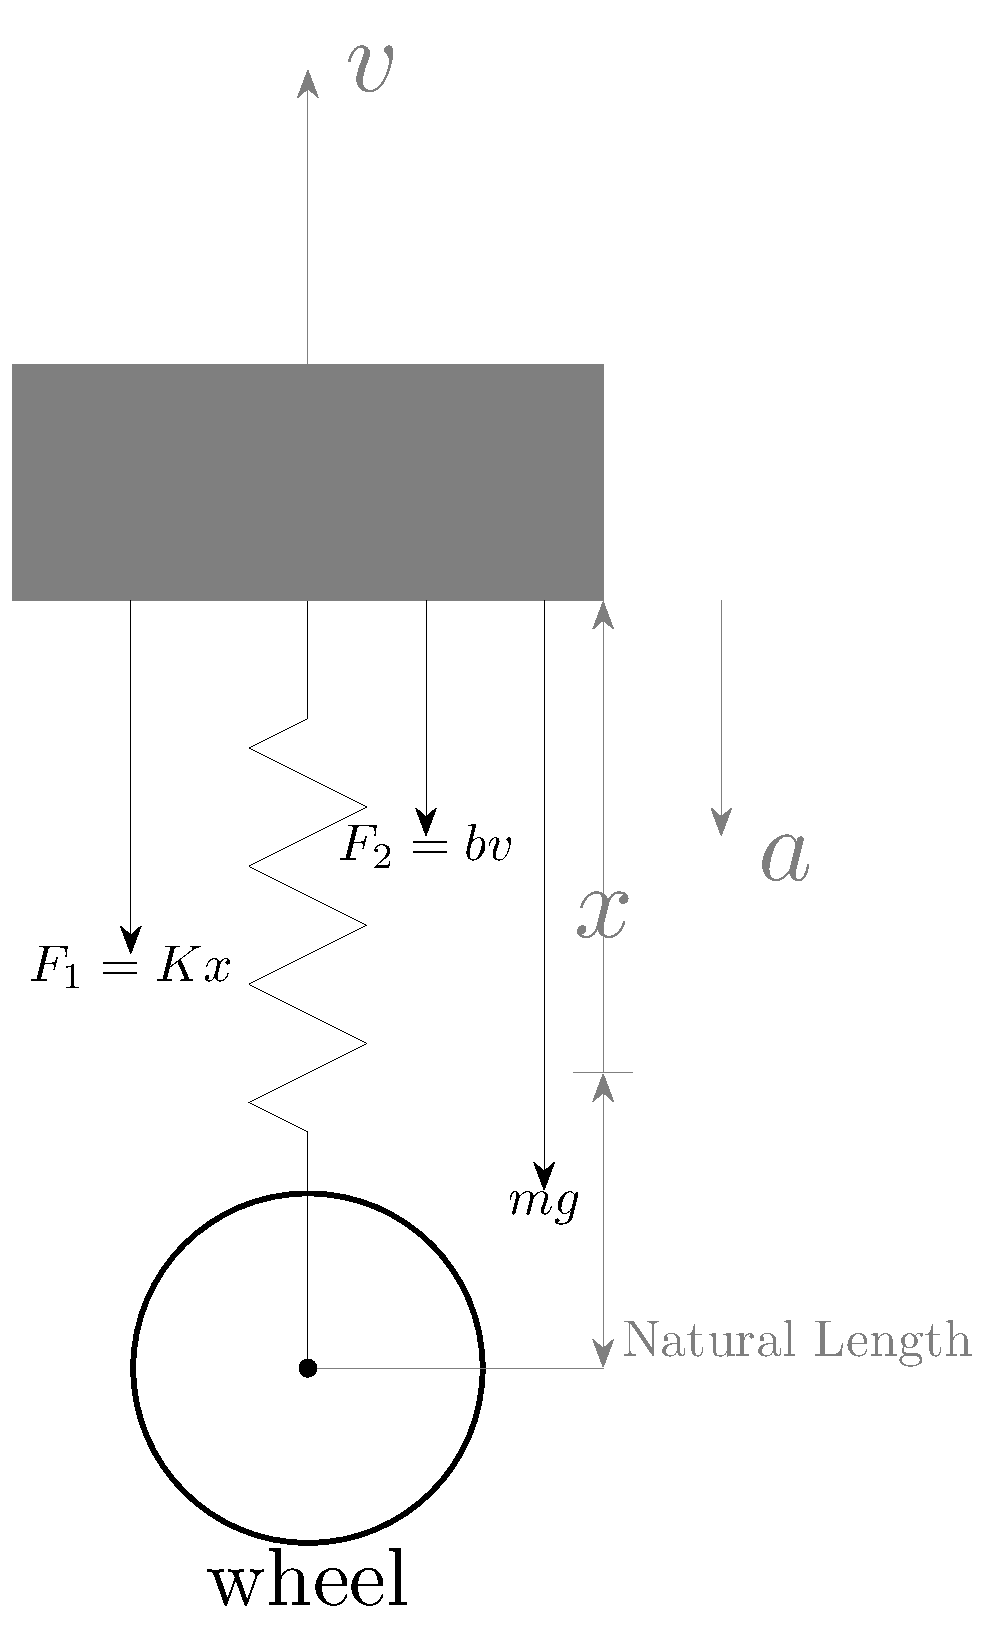
\includegraphics[width=0.3\linewidth]{11_14_21_fbd.pdf}
        \caption{FBD of the damped oscillation system}
        \label{fig:enter-label}
    \end{figure}
\item \textbf{Eqn:}
From the FBD of the system we can write the force equation,
\begin{align}
    &F=F_{1}+F_{2}\\
    \Rightarrow&F=Kx+bv\\
    \Rightarrow&ma=kx+bv\\
    \Rightarrow&-m\frac{d^2x}{dt^2}=kx+b\frac{dx}{dt}\\
    \Rightarrow&\frac{d^2x}{dt^2}+\left(\frac{b}{m}\right)\frac{dx}{dt}+\frac{k}{m}x=0
\end{align}
\end{enumerate}   

\end{document}


